\subsection{DNA Cloning}
The transformation with the new constructs was validated by sequencing following the mini-preparation. All clones showed 100\% sequence identity with the designs. The concentrations of the plasmids after the midi preparation were measured as \SI{605}{\nano\gram\per\micro\litre} (d29-A), \SI{335}{\nano\gram\per\micro\litre} (S-Tag-A), and \SI{300}{\nano\gram\per\micro\litre} (S-Tag-B), corresponding to yields of \SI{302}{\micro\gram}, \SI{167}{\micro\gram}, and \SI{150}{\micro\gram}.

\subsection{Protein Analysis}
\subsubsection{eYFP Yield by Fluorescence}
For an estimate of the protein yield in the lysate, a fluorescence analysis of a cell-free expression setup expressiong Strep-eYFP was conducted. The calibration showed a linear trend with a coefficient of determination of $R^2 = 0.98$ (\autoref{fig:calibration_eyfp}). Applying the linear model to the sample values, the concentration of Strep-eYFP in the lysate was estimated as \SI{295}{\micro\gram\per\milli\litre}.

\subsubsection{Coomassie Staining and Western Blot} 
Coomassie staining and Western Blot were conducted both directly after the cell-free expression and after the following CaptoCore purification. For each setting, two blots were developed, one using an anti-PVX antibody, and one using an anti-S-Tag antibody. 

For the samples from cell-free expression (\autoref{fig:blot_alice}), the Coomassie Staining shows a wide range of bands. For the samples from ALiCE setups expressing d29-A, S-Tag-A, and S-Tag-B, the pattern looks very similar to that of the non-template control. The sample expressing Strep-eYFP has a notable band at a height corresponding to ~\SI{30}{\kilo\dalton}, similar to the single band in the Strep-eYFP control. The track containing the S-Tag-CP-PVX control also displays a single band at ~\SI{29}{\kilo\Dalton}, slightly lower than that of the Strep-eYFP control. The sample from the ALiCE setup expressing PVX CP presents a band ~\SI{29}{\kilo\dalton} as well. 

In the Western Blot based on the anti-PVX antibody, the samples from the ALiCE expressions of d29-A, S-Tag-A, and PVX CP show strong bands at ~\SI{25}{\kilo\Dalton}, ~\SI{31}{\kilo\Dalton}, and ~\SI{29}{\kilo\Dalton}. The band for the expressed PVX CP is particularly strong. The sample from S-Tag-B shows a faint band at ~\SI{28}{\kilo\Dalton}. The control S-Tag-CP-PVX has two bands visible in the blot, a stronger band at ~\SI{28}{\kilo\Dalton}, and a less prominent one at ~\SI{30}{\kilo\Dalton}. In all samples, the observed bands migrated to higher molecular weights than the theoretical molecular weights of \SI{22.6}{\kilo\Dalton} (d29-A), \SI{26.9}{\kilo\Dalton} (S-Tag-A), \SI{26.8}{\kilo\Dalton} (S-Tag-B), \SI{25.1}{\kilo\Dalton} (CP-PVX), and \SI{26.9}{\kilo\Dalton} (S-Tag-CP-PVX).

In the blot using the anti-S-Tag antibody, the tracks containing samples from the expression of S-Tag-A and S-Tag-B show a strong signal. For S-Tag-A, the blot shows strong lines at ~\SI{31}{\kilo\Dalton}, ~\SI{29}{\kilo\Dalton}, and ~\SI{28}{\kilo\Dalton}, but with a fainter, diffuse trail to higher and lower molecular weights. In the track containing S-Tag-B, there are prominent lines visible at molecular weights of ~\SI{29}{\kilo\Dalton}, ~\SI{28}{\kilo\Dalton}, and ~\SI{25}{\kilo\Dalton}, as well as a faint, diffuse trail similar to that of S-Tag-A. The control containing S-Tag-CP-PVX shows a strong band at ~\SI{32}{\kilo\Dalton} and a faint band at ~\SI{30}{\kilo\Dalton}.

The Coomassie Gel of the samples after the CaptoCore chromatography (\autoref{fig:blot_capto}) shows no bands except for the control S-Tag-PVX-CP, which has a band at ~\SI{30}{\kilo\Dalton}. The blot using anti-PVX antibodies shows a faint band for the sample of purified S-Tag-A at ~\SI{31}{\kilo\Dalton} and for the sample of purified PVX CP at ~\SI{30}{\kilo\Dalton}. The control containing S-Tag-PVX-CP particles has bands two bands at ~\SI{30}{\kilo\Dalton} and ~\SI{34}{\kilo\Dalton}. In the blot using the anti-S-Tag antibody, the sample from S-Tag-A shows a faint line at ~\SI{31}{\kilo\Dalton}. The track of the sample from S-Tag-B has a very faint line at ~\SI{30}{\kilo\Dalton}. The control S-Tag-PVX-CP has two bands, a strong one at ~\SI{35}{\kilo\Dalton} and a fainter one at ~\SI{33}{\kilo\Dalton}. 


\begin{figure}
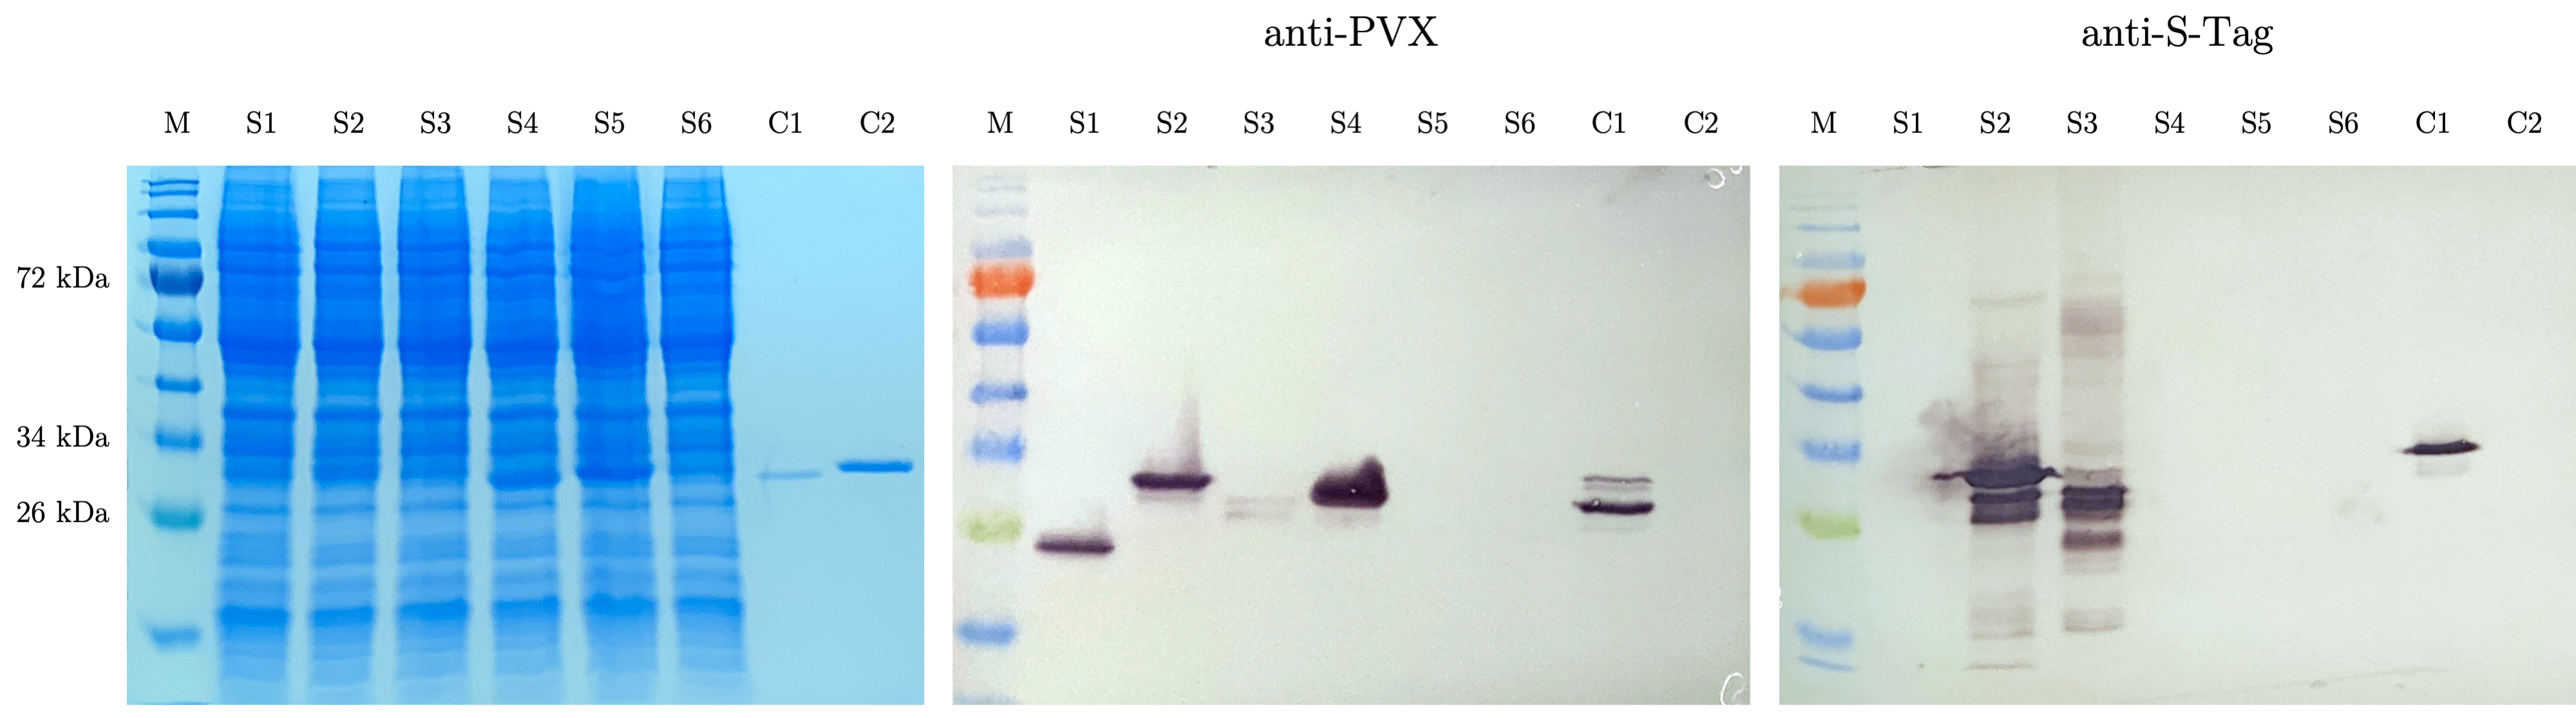
\includegraphics{lab/blot_alice.png}
\caption{\text{Coomassie Gel and Blot images following ALiCE expression.}}
\label{fig:blot_alice}
\end{figure}
\begin{figure}
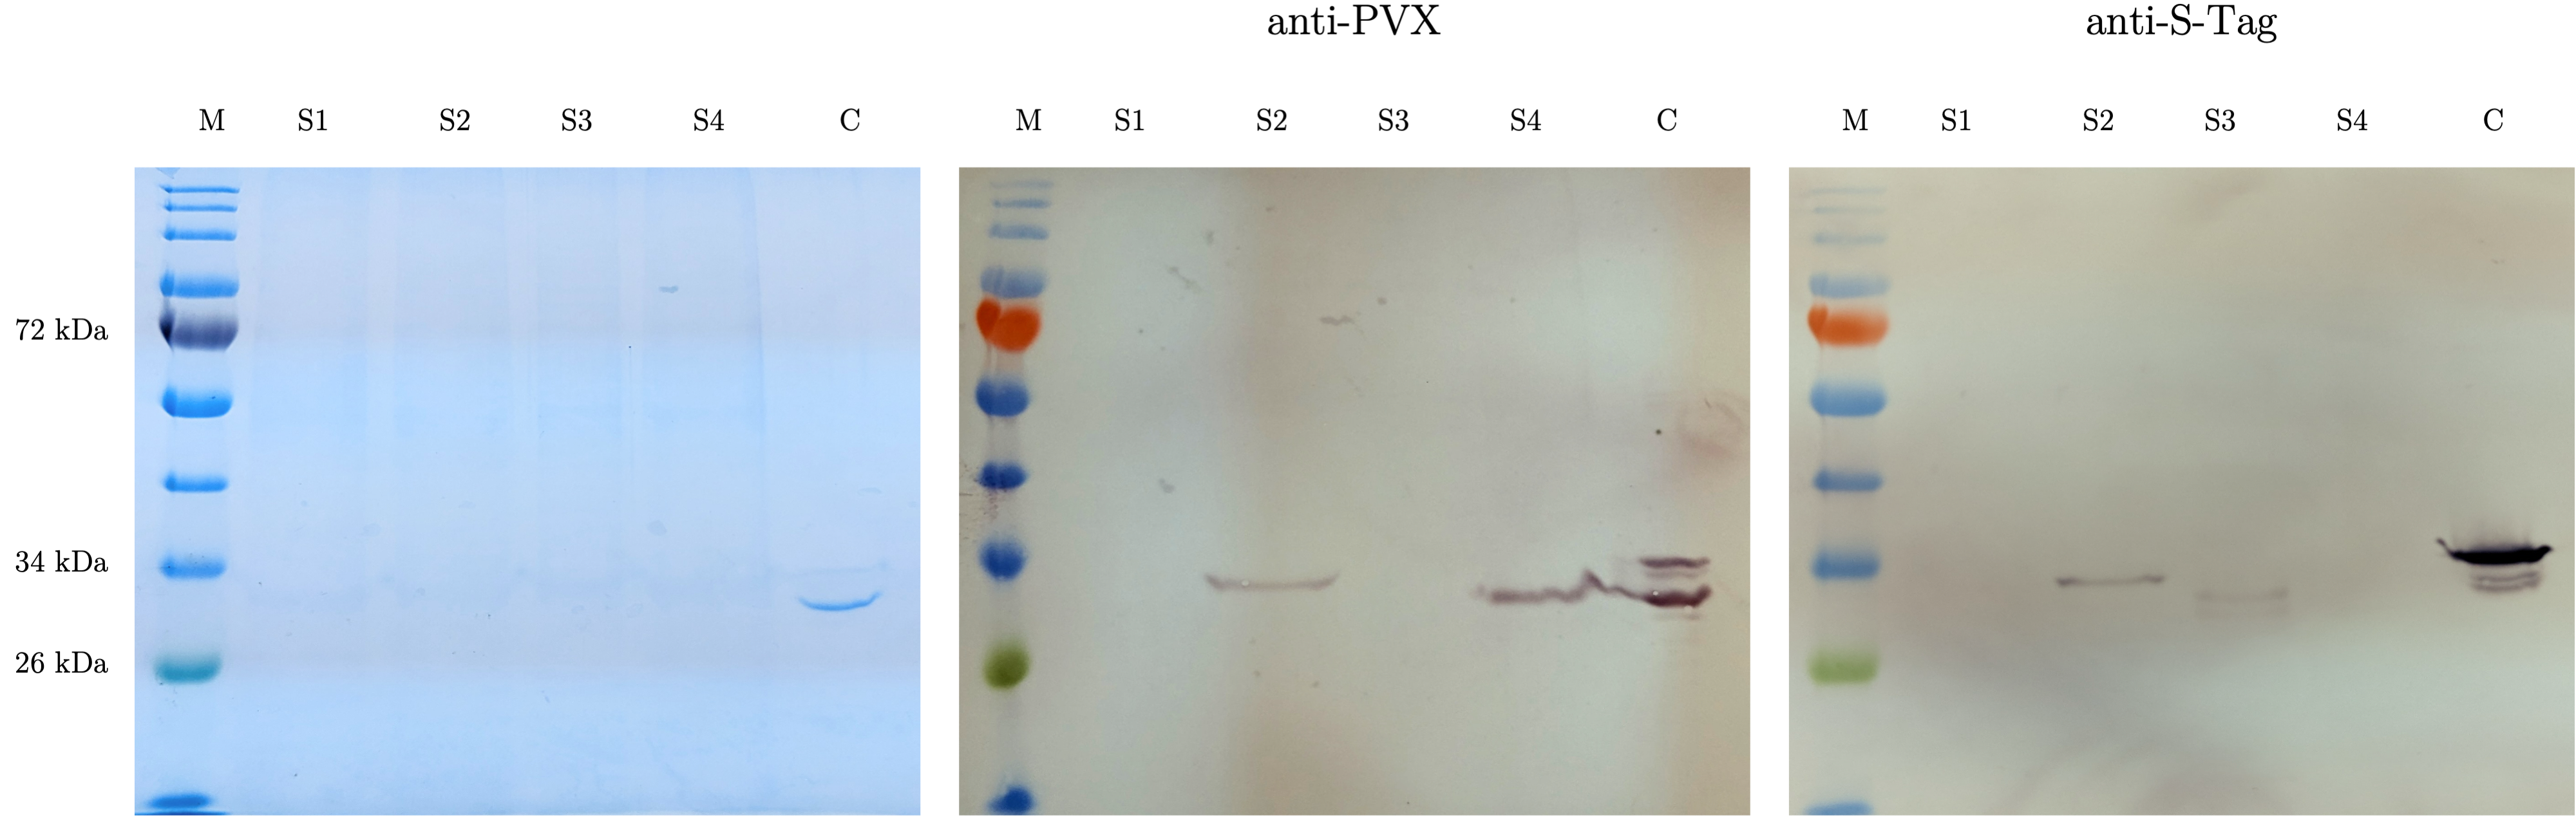
\includegraphics{lab/blot_capto.png}
\caption{\text{Coomassie Gel and Blot images following CaptoCore Purification.}}
\label{fig:blot_capto}
\end{figure}


\subsubsection{ELISA}
For a quantitative analysis of the cell-free protein expression, an ELISA was performed on the samples, using both the anti-PVX antibody, and the anti-S-Tag antibody. 

The calibration measurements for the anti-PVX-antibody show saturation at protein concentrations larger than \SI{100}{\nano\gram\per\milli\litre}. The four calibration samples below that threshold follow a linear trend 
\begin{equation}
\text{OD} = \SI{6.5}{\micro\litre\per\nano\gram} \cdot c
\end{equation}
with a coefficient of determination of $R^2=0.90$ (\autoref{fig:elisa_calib}). The measurements from the samples yielded significant OD values for d29-A, S-Tag-A, and CP-PVX, and no significant signal for S-Tag-A and the non-template H\textsuperscript{2}O from the ALiCE expressions (\autoref{tab:sample_values_elisa_anti_pvx}). For d29-A, S-Tag-A, and CP-PVX, the measured ODs of the different dilutions were almost identical, with an OD of ~0.2 for d29-A, 0.22 for S-Tag-A, and ~0.87 for CP-PVX. Due to this, the back-calculated concentrations using the linear model and the dilution factors vary over the two dilutions. Calculations based on the stronger diluted samples yield to concentrations of \SI{30\pm 5}{\micro\gram\per\milli\litre} for d29-A, \SI{33\pm 4}{\micro\gram\per\milli\litre} for S-Tag-A, and \SI{134\pm 4}{\micro\gram\per\milli\litre} for CP-PVX. 

For the anti-S-Tag antibody, calibration was sub-linear for low concentrations, but followed a linear trend for the whole sample range up to \SI{1500}{\nano\gram\per\milli\litre}. The linear model was calculated as 
\begin{equation}
\text{OD} = \SI{0.9}{\micro\litre\per\nano\gram} \cdot c
\end{equation}
and yielded a coefficient of determination of $R^2 = 0.98$ (\autoref{fig:elisa_calib}). As for the anti-PVX-antibody, the sample OD measurements were highly similar for the 1:500 and 1:1000 dilutions (\autoref{tab:sample_values_elisa_anti_s_tag}), with significant ODs of 2.4/2.2 (1:500/1:1000)  for S-Tag-A and 1.5/1.1 (1:500/1:1000) for S-Tag-B. The samples of d29-A, CP-PVX, and the non-template control showed no significant absorbtion. Following back-calculation of the stronger dilution, the concentration for S-Tag-A was evaluated as \SI{2400\pm 90}{\micro\gram\per\milli\litre}, and for S-Tag-B as \SI{1200\pm 100}{\micro\gram\per\milli\litre}.

\subsubsection{Electron Microscopy}